% Also try the document class 'amsart'.
\documentclass[a4paper, oneside, onecolumn, 11pt, notitlepage, reqno]{article}

% Load preamble
\usepackage{kvalheimracing}
\usepackage[lmargin=2cm, rmargin=2cm, tmargin=2cm, bmargin=2cm]{geometry}

% Hyperref setup
\hypersetup{pdfauthor={Eirik Kvalheim}}
\hypersetup{pdftitle ={Document Title}}

\title{Leiekontrakt for utleie av Næringslokale}
\author{Hjeravegen 999}
\date{Mai, 2020}

%\setcounter{secnumdepth}{3}

%\renewcommand*\contentsname{Innhold}
\renewcommand\maketitlehooka{\null\mbox{}\vfill}
\renewcommand\maketitlehookd{\vfill\null}
\renewcommand{\figurename}{Vedlegg}

\newcommand{\namesig}[2][7cm]{
  \begin{tabular}{@{}p{#1}@{}}
	#2 \\\\[2\normalbaselineskip] \noindent\rule{7cm}{0.4pt} \\[0pt]
	{\small \textit{Navn med blokkbokstaver}} \\\\[2\normalbaselineskip] \noindent\rule{7cm}{0.4pt} \\[0pt]
	{\small \textit{Signatur}}
  \end{tabular}
}


\begin{document}

	\begin{titlingpage}
		\maketitle
	\end{titlingpage}

%	\tableofcontents

	\section{PARTENE} \label{Sec: PARTENE}


    \begin{enumerate}


        \item Utleier\\Eirik Kvalheim\\230591*****\\Hjeravegen 999, 2072 Dal

        \item Leietaker\\Ola Normann\\31019532456\\Org. nr. 999999999


    \end{enumerate}

	\section{EIENDOM}


    \begin{enumerate}


        \item Hjeravegen 164, 2072 Dal\\Gr.nr 93 br.nr 100\\Eidsvoll kommune, nr. 3035

    \end{enumerate}

	\section{LEIEOBJEKT}


	\begin{enumerate}


		\item Arealer til leietakers bruk er: ca. 80 kvm. BTA

		\item Eventuelle feil i arealangivelsene gir ikke rett til å kreve leien justert, og medfører heller ikke noen endring av
		denne leieavtales øvrige bestemmelser

		\item Det er stor plass for flere midlertidige parkeringer utenfor lokalet. Her gjelder for leietaker "parkering på eget ansvar", da utleier leier ut containere som benyttes til lagerplass, og dersom leietakere av containerne trenger tilgang til disse må dette gis umiddelbart. Leietaker oppfordres til å leie en eller flere containere for å skaffe seg faste parkeringsplasser på området

		\item Det er felles snuplassområder i nabolaget, og leietaker står fritt til å snakke med naboer i forhold til å bruke denne til midlertidige parkeringsplasser, da dette har blitt gjort av tidligere leietakere

		\item Følgende er mulige utvidelser som utleier vil dekke 50\% av kostnaden på, mot at utvidelsene tilfaller leieobjektet og utleiers eie:

			\begin{enumerate}

				\item Installasjon i lokalet av skruekompressor m. lufttørke, rørsystem, slangetromler hengende fra taket og luftuttak langs veggen. Dette systemet vil forsyne begge verkstedlokalene som er vegg i vegg

				\item Bygging av sliperom under hems. Det er tiltenkt at man tetter igjen åpningen mot reolene og henger opp svart sveiseforheng med gardintype oppheng for å ha muligheten til å dekke åpningen mot løftebukken. Installasjon av "disk-sander", båndsliper, skrustikke og slipebord

				\item Generell utbedring av ventilasjonsanlegg og spesielt tillegg med egen eksosventilasjon

				\item Materialkappesag for alt av metaller

				\item Sandblåsekabinett med installasjon

				\item Hydraulisk presse

				\item Søylebormaskin

				\item Plasmakutter

			\end{enumerate}

			Disse utvidelsene vil projekteres og styres av utleier, og leietaker plikter og sette seg inn i og benytte seg av brukerinstrukser og manualer for medfølgende utstyr. Hvorvidt utvidelsene igangsettes eller ikke avgjøres av utleier, dersom leietaker ønsker en utvidelse

		\item Leieobjektet er vegg i vegg med utleiers eget verksted, og det benyttes en felles hoveddør

		\item På sommeren er det anledning til å benytte seg av bygningens utekran for varmt og kaldt vann, for vasking av biler eller lignende. Det fins stikkontakt utenfor til bruk av f.eks høytrykkspyler

		\item Inkludert i leieobjektet er følgende:

			\begin{itemize}

				\item 3 Seter skinnsofa

				\item Whiteboardtavle

				\item Veggmonterte ovner på tilsammen 2,4kW

				\item Wi-Fi. Hastighet og stabilitet kan variere som følge av nettverksproblemer fra teleselskapet

				\item 42" TV og Chromecast

				\item Brannslukningsaparater

				\item Alarmanlegg med brannvarsler og vekterutrykning

				\item Elektronisk kodelås med app

				\item Punktavsug

				\item Metallhylle

				\item Jekketralle

				\item Reoler

			\end{itemize}

		\item Vask og kjøleskap i utleiers verksted kan benyttes. Det er ikke anledning for å låne noe, ta noe, eller benytte seg av noe som helst annet i utleiers eget verksted. Det spesifiseres at dette godet forutsetter en gjensigig tillit og god kommunikasjon. Dersom utleier vurderer det dithen at dette ikke forekommer kan leietaker miste tilgangen til bruk av vask og kjøleskap. Dette vil f.eks forekomme dersom verktøy eller utstyr blir stålet, vask eller kjøleskap tilgriset uten vilje til å rengjøre, eller ved oppdagelse av personer på andre steder som de ikke skal være i utleiers eget verksted. Vask og kjøleskap skal etter hver gangs bruk forlates i like god eller renere tilstand enn før man benyttet det

		\item Toalett medfølger ikke, men det er i utleiers kontorbygg et toalett. Mellom kl 8 og kl 18 er det anledning til å banke på døren og spørre om å låne toalettet. Dersom toalettet forlates i like god eller renere tilstand er det svært liten sansynlighet for å få et "nei" ved neste trengende anledning

		\item Varmen i lokalet er den som kan genereres av de tre ovnene på tilsammen 2,4kW

	\end{enumerate}

	\section{LEIETAKERS VIRKSOMHET}


	\begin{enumerate}


		\item Det er ingen spesielle krav til formål og virksomhet ved benyttelse av leieobjektet annet enn neste delpunkt, samt at virksomheten skal være lagrings og/eller verksted relatert

		\item Endring av virksomheten i leieobjektet, herunder drift av annen, beslektet virksomhet, er ikke tillatt uten utleiers skriftlige forhåndssamtykke. Samtykke kan ikke nektes uten saklig grunn. Økt avgiftsmessig belastning for utleier som følge av leietakers
		endrede virksomhet skal anses som saklig grunn, med mindre leietaker forplikter seg til å holde utleier skadesløs for tleiers tap
		og kostnader og stiller en – etter utleiers oppfatning – tilfredsstillende sikkerhet for sine forpliktelser. Videre skal opprettholdelse
		av eiendommens virksomhetsprofil/virksomhetssammensetning anses som saklig grunn


	\end{enumerate}

	\section{OVERTAKELSE}


    \begin{enumerate}

    	\item Leieobjektet overtas inklusive inventar og utstyr, ryddet og rengjort, og for øvrig i den stand som
        leieobjektet var i ved leietakers besiktigelse den 99.99.2020

    	\item Leietaker må gi skriftlig melding om mulige skader og mangler m.v. innen rimelig tid etter at han/hun
        burde ha oppdaget dem. Med rimelig tid defineres all tid kortere enn tre dager. Forhold som leietaker kjente til ved overtakelsen, kan ikke senere gjøres gjeldende som mangel

        \item Ved overtakelse skal utleier gi leietaker en innføring i bruk av teknisk utstyr og innretninger i leieobjektet som skal benyttes av leietaker. Spesielt gjelder dette kjøretøyløfter, ventilasjonsanlegg og elektronisk dørlås, men også IT momenter som nettverk og diverse apper.

        %Videre skal Utleier ved Overtakelse fremlegge driftsmanualer/-instrukser for teknisk utstyr og innretninger i Leieobjektet. Leietaker skal i hele Leieperioden følge Utleiers til enhver tid gjeldende driftsmanualer/-instrukser.

    \end{enumerate}

	\section{LEIETID}


	\begin{enumerate}

		\item Leieforholdet løper fra Juni 2020 til og med August 2022, hvoretter leieforholdet opphører uten oppsigelse

		\item Det er ikke er oppsigelsesadgang i leieperioden

	\end{enumerate}

	\section{LEIESUM}


	\begin{enumerate}


        \item Leien forfaller til betaling forskuddsvis den 10. hver måned med NOK 9500,-

		\item Unntak fra punkt 7.1 gjelder de tre første månedene hvor det gis rabatter. Første måned betales 25\% av leieprisen, andre måned 50\% av leieprisen, og tredje måned 75\% av leieprisen. Fra og med fjerde måned betales full leiepris

		\item Strøm, alarm med vekterutrykning, internett og vanlig søppelforbruk er inkludert i leieprisen definert i punkt 7.1 og 7.2

        \item Leien innbetales til utleiers konto nummer 12017181651

		\item Betaling anses ikke skjedd før NOK 9500,- er mottatt på utleiers konto

		\item Unntak fra punkt 7.5 gjelder de tre første månedene

		\item Dersom leietaker krever vann til annet enn vanlig renhold o.l., må utleiers
        samtykke innhentes. Samtykke kan ikke nektes uten saklig grunn. Et månedlig vanngebyr vil påløpe dersom leietaker får samtykke til et slikt krav

		\item I den grad utleie av eiendom blir belagt med særlige skatter og/eller avgifter, skal leietaker betale sin
        forholdsmessige del etter leie som nevnt i dette punkt 7 første avsnitt

		\item Ved forsinket betaling av leie, svares forsinkelsesrente i henhold til lov av 17. desember 1976 nr. 100 eller lov som trer i stedet for denne. Utleier har rett til å kreve gebyr på NOK 100,- ved purring


	\end{enumerate}

	\section{LEIETAKERS BENYTTELSE AV LEIEOBJEKTET}


    \begin{enumerate}


        \item Leietaker plikter å sette seg inn i og følge de offentlige forskrifter, vedtekter, instrukser, ordensregler
        o.l. som er eller måtte bli innført og som kommer til anvendelse på leieforholdet. Leietaker er ansvarlig
        overfor alle offentlige myndigheter for at hans benyttelse av leieobjektet tilfredsstiller de til enhver tid
        gjeldende offentligrettslige krav. Alle offentligrettslige krav, herunder krav fra arbeidstilsyn, helseråd,
        sivilforsvar, industrivern, brannvern, statens vegvesen eller annen offentlig myndighet, foranlediget av den virksomhet som
        drives i leieobjektet, er det leietakers ansvar å oppfylle per overtakelse og for øvrig i leieperioden

        \item Leieobjektet må ikke benyttes på en måte som forringer eiendommens omdømme eller utseende eller
        ved støv, støy, lukt, rystelse eller på annen måte sjenerer andre leietakere eller naboer. Kostnadene ved utbedring og eventuell
        erstatning i forbindelse med disse forhold, er leietakers ansvar

        \item Det henvises til normale regler om ro etter kl 20:00. Det kan drives virksomhet hele døgnet, men etter kl 20:00 bes det om å bruke skjønn med tanke på bråk og støy, spesielt av dype frekvenser. Det er ikke lov å drive med motortuning og støyfull motortesting mellom kl 20:00 og kl 08:00

        \item Det er ikke anledning til å koble på flere elektriske ovner enn det som allerede finnes i lokalet. Ved behov for mer varme eksempelvis som følge av åpen port på vinterstid, må det benyttes jetvarmer eller annen varmer på eget drivstoff. Denne skal ikke stå på uten oppsyn

        \item På vinteren må leietaker selv stå for måking. Det blir satt ut snøskuffer utenfor bygningen som kan benyttes. Det skal ikke måkes snøhauger foran containerne eller utleiers område

        \item Urinering på eiendommens område er ikke tillatt

        \item Tildekning av ovner er ikke tillatt

        \item Avfall må legges i lokalets søppelkasse. Hverken søppelkassen, løst søppel, eller deler fra leietaker skal befinne seg utenfor lokalet.
        Det skal benyttes gjennomsiktige søppelposer som dagen før avfallshenting kan settes ved nabolagets søppelkasser. Avfallet gjelder som restavfall. Appen "Min Renovasjon" må benyttes for informasjon og varsling om lokalets tømmekalender. Det er ikke anledning til å sette mer enn én full søppelpose for henting per tømmedag. Søppelposen skal knytes godt igjen.
        Avfall utover én full søppelsekk eller av ekstraordinært omfang, må leietaker selv besørge fjernet for egen regning.
        Leietaker må selv sørge for tømming av oljefat når dette er fullt, og ved utflyning av lokalet

        \item Røyking er forbudt inne i lokalet. Ved røyking utenfor lokalet skal port samt hoveddør være lukket og askebeger på veggen skal benyttes for sneiper. Leietaker eller leietakers bekjente skal aldri kaste løse sneiper eller snusposer rundt omkring på eiendommen


    \end{enumerate}

	\section{UTLEIERS ADGANG TIL LEIEOBJEKTET}


    \begin{enumerate}


        \item Leietaker plikter å gi utleier adgang til leieobjektet alle dager, for ettersyn,
        reparasjon, vedlikehold, inspeksjon, taksering, forandringsarbeid etc.
        I alle tilfeller der det anses nødvendig for å forebygge eller begrense skade på eiendommen, har
        utleier rett til å skaffe seg adgang til leieobjektet uten slikt varsel

        \item Utleier har adgang til bruk av lokalet med kjøretøyløfter for egne korte arbeider, men leietaker har primærrett til bruk av lokalet. Det planlegges mulige utvidelser som utleier vil ta del i å installere, og disse utvidelsene vil utleier benytte seg av, spesielt et eventuelt sliperom

        \item Utleier får benytte seg av to palleplasser i pallereolene til lagring

    \end{enumerate}

	\section{UTLEIERS VEDLIKEHOLDSPLIKT}


    \begin{enumerate}

        \item Det påhviler utleier å besørge og bekoste alt utvendig bygningsmessig vedlikehold. Likeledes påhviler
        det utleier å skifte ut tekniske innretninger anbragt av utleier, slik som ventilasjonsanlegg,
        branntekniske anlegg, alarmanlegg etc., når disse ikke lenger lar seg vedlikeholde på regningssvarende
        måte

        \item Det påhviler utleier å besørge at bygningen med tekniske innretninger holdes i tilsvarende stand som
        ved kontraktsinngåelsen, eller bedre, dog slik at alminnelig slitasje må aksepteres av leietaker

        \item Avbrudd som ikke er vesentlige, i forsyninger av vann, strøm, luft etc., plikter leietaker å tåle uten
        erstatning eller avslag i leien

    \end{enumerate}

	\section{LEIETAKERS VEDLIKEHOLDSPLIKT}


    \begin{enumerate}

        \item Leietaker plikter å behandle så vel leieobjektet som eiendommen for øvrig med tilbørlig aktsomhet

        \item Det påhviler leietaker å besørge og bekoste vedlikehold av leieobjektet, herunder også ut- og innvendig
        vedlikehold av inngangsdør og port samt innvendig vedlikehold, slik at
        alt er i forskrifts- og håndverksmessig god stand. Vedlikeholdsplikten for leietaker omfatter også
        fornyelse av gulvbelegg og annen oppussing og istandsetting innvendig, herunder
        overflatebehandling av gulv, vegger og tak. Videre omfatter vedlikeholdsplikten de i lokalet synlige rør,
        ledninger og installasjoner tilknyttet forsyning av vann, luft, varme og elektrisitet, og
        ventilasjon. Det påhviler likeledes leietaker å besørge og bekoste vedlikehold og utskiftning
        av inventar og utstyr som medfølger leieobjektet. Utleier har ikke ansvar for vedlikehold eller utskiftning
        av innretninger anbragt i leieobjektet av leietaker. Alt arbeid leietaker plikter å utføre, skal han foreta uten
        ugrunnet opphold, med normale intervaller i leieperioden og på en håndverksmessig god måte

        \item Leietakers vedlikeholdsplikt omfatter også skader etter innbrudd og/eller hærverk i leieobjektet,
        herunder skader på inngangsdør og port

        \item Leietaker plikter å sørge for reparasjon og vedlikehold av de skilt etc. som utleier har gitt tillatelse til å
        sette opp

        \item Oppfyller ikke leietaker sin vedlikeholdsplikt er utleier berettiget til, etter skriftlig varsel med 14
        dagers oppfyllelsesfrist, å utføre vedlikeholdsarbeidene for leietakers regning



    \end{enumerate}

	\section{UTLEIERS ENDRING AV LEIEOBJEKTET}


    \begin{enumerate}


        \item Utleier er berettiget til å foreta alle arbeider som måtte være nødvendige til eiendommens forsvarlige
        vedlikehold eller fornyelse, og til i samme utstrekning å foreta ethvert forandringsarbeid (herunder
        tilbygg, påbygg m.v.) såvel i som utenfor leieobjektet. Leietaker plikter å medvirke til at ledninger,
        kanaler og rør etc. til andre deler av eiendommen, kan føres gjennom leieobjektet uten hinder av
        leietakers innredning

        \item Leietaker plikter å finne seg i slike arbeider uten erstatning eller avslag i leien, med mindre ulempene
        for ham er vesentlige. Utleier skal påse at arbeidene blir til minst mulig sjenanse for leietaker. Leietaker
        skal varsles med rimelig frist

        \item Utgifter i forbindelse med offentlige krav om forhøyet teknisk standard som måtte pålegges utleier i
        leieperioden, kan utleier kreve dekket hos leietaker i den utstrekning tiltaket kommer leietaker til gode


    \end{enumerate}

	\section{LEIETAKERS ENDRING AV LEIEOBJEKTET}


    \begin{enumerate}


        \item Leietaker kan ikke foreta bygningsmessig forandring i eller av leieobjektet uten
        utleiers skriftlige forhåndssamtykke, som også kreves om leietaker ønsker å bruke mer strøm, vann,  m.v. enn
        hva leieobjektet ved kontraktstidspunktet var utstyrt med. Samtykke kan ikke nektes uten saklig grunn.
        Spesielt kan man på ingen måte endre sammensetningen av pallereolene

        \item Radio- og høytaler-anlegg m.v., store skap, automater o.l. må ikke settes opp uten utleiers skriftlige
        forhåndssamtykke. Samtykke kan nektes på fritt grunnlag

        \item Endringsarbeider beskrevet i dette punkt 13 tilfaller utleier etter endt leieperiode, med mindre utleier
        forlanger leieobjektet satt tilbake i sin opprinnelige stand

        \item Leietaker er ansvarlig for å innhente de nødvendige offentlige tillatelser for eventuelle arbeider som
        utføres i henhold til dette punkt 13


    \end{enumerate}

	\section{FORSIKRING}


    \begin{enumerate}

        \item Hver av partene holder sine interesser forsikret

        \item Utleier forsikrer bygningen

        \item Leietaker forsikrer egen bygningsmessig innredning, fast og løst inventar, løsøre, maskiner, data, varer,
        driftstap/avbrudd og ansvar. Skade påført leietakers medkontrahenter som følge av avbrudd, forsinkelser eller
        oppgjør i henhold til bestemmelsene i dette punkt 14, er leietakers ansvar. Ved skade på leieobjektet skal
        leietakers forsikring benyttes så langt den dekker, inkludert mulig egenandel, før utleiers forsikring
        benyttes

        \item Medfører leietakers virksomhet forhøyelse av eiendommens forsikringspremier eller faste avgifter,
        eller pålegg fra utleiers forsikringsselskap om investeringer, plikter leietaker å dekke kostnaden.
        Leietaker plikter å melde til utleier ethvert forhold og/eller endring i forhold ved virksomheten, som kan
        få følger for eiendommens forsikringspremie. Utleier har ikke ansvar for skader eller tap som måtte
        oppstå ved innbrudd, brann, vannskade m.v., ut over det som omfattes av de forsikringer utleier har som
        huseier

        \item Partene kan kreve at den annen part legger frem forsikringsbevis med vilkår og kvittering for betalt
        forsikring. Partenes rettslige posisjon skal ikke påvirkes av om forsikringsbevis/kvittering er fremlagt
        eller ikke

    \end{enumerate}

	\section{BRANN ELLER DESTRUKSJON}


    \begin{enumerate}

        \item Blir leieobjektet ødelagt ved brann eller annen hendelig begivenhet kan utleier erklære seg fri fra alle
        rettigheter og forpliktelser under leieavtalen

    \end{enumerate}

	\section{UTLEIERS AVTALEBRUDD}


    \begin{enumerate}


        \item Leietaker kan kreve avslag i leien i henhold til husleieloven § 2-11 som følge av forsinkelse eller
        mangel. Hva gjelder mangel, forutsettes at mangelen er vesentlig og at mangelen ikke rettes av utleier i henhold
        til bestemmelsene i husleieloven § 2-10. Denne bestemmelse gjelder både
        forsinkelse/mangler pr. overtakelse og mangler i leietiden. Leietaker må gi skriftlig melding om skader og mangler
        mv. innen rimelig tid etter at leietaker burde ha oppdaget dem. Rimelig tid er definert i punkt 5.2

        \item Leietaker har ikke rett til å holde tilbake leie til sikkerhet for de krav leietaker har eller måtte få mot utleier som følge av mangel eller forsinkelse

        \item Leietaker kan kreve erstatning for direkte tap som følge av forsinkelse eller mangel i henhold til
        husleieloven § 2-13. Hva gjelder mangel, forutsettes at mangelen er vesentlig og at mangelen ikke rettes av
        utleier i henhold til bestemmelsene i husleieloven § 2-10. Indirekte tap dekkes ikke.
        Erstatningens størrelse begrenses oppad til ett kvartals leie, med mindre utleier har handlet forsettlig
        eller grovt uaktsomt. Denne bestemmelse gjelder både forsinkelse/mangler pr. overtakelse og mangler i
        leietiden

        \item Dersom leietaker ønsker å påberope vedvarende eller gjentatt mislighold fra utleiers side som grunnlag
        for heving, se for øvrig kravene i husleieloven § 2-12, krever dette skriftlig forhåndsvarsling om at avtalen
        kan bli hevet om misligholdet ikke opphører


    \end{enumerate}

	\section{LEIETAKERS AVTALEBRUDD}


    \begin{enumerate}


        \item Leietaker blir erstatningsansvarlig for all skade eller mangler som skyldes ham selv eller folk i hans
        tjeneste, faste eller tilfeldige, samt fremleietakere, kunder, leverandører og/eller andre personer som han
        har gitt adgang til eiendommen. Erstatningsplikten omfatter også utgift som måtte følge av utrydding av
        utøy

        \item Leietaker vedtar at tvangsfravikelse kan kreves hvis leien eller avtalte tilleggsytelser ikke blir betalt, jf.
        § 13-2 3. ledd (a) i tvangsfullbyrdelsesloven. Leietaker vedtar at tvangsfravikelse kan kreves når leietiden
        er løpt ut, jf. § 13-2 3. ledd (b) i tvangsfullbyrdelsesloven. Ved vesentlig mislighold som ikke gjelder manglende betaling og fraflytting kan utleier benytte seg av lov om tvangsfullbyrdelse § 13-2, 3. ledd pkt. c, d og e

        \item Gjør leietaker seg skyldig i vesentlig mislighold av leieavtalen kan utleier heve denne, og leietaker
        plikter da å fraflytte leieobjektet

        \item En leietaker som blir kastet ut eller flytter etter krav fra utleier pga. mislighold eller fraviker
        leieobjektet som følge av konkurs, plikter å betale leie (og eventuelle øvrige betalingsforpliktelse under
        leieavtalen) for den tid som måtte være igjen av leietiden. Betalingsplikten suspenderes for den periode
        utleier får leid ut leieobjektet på ny, til samme eller høyere pris. Leietaker må også betale de
        omkostninger som utkastelse, søksmål og rydding/rengjøring av leieobjektet fører med seg, samt utgifter
        til ny utleie


    \end{enumerate}

	\section{FRAFLYTTING}


    \begin{enumerate}

        \item Ved fraflytting skal utleier umiddelbart gis adgang til leieobjektet

        \item Leietaker skal ved fraflytting tilbakelevere leieobjektet ryddiggjort, rengjort og
        for øvrig i kontrakts- og håndverksmessig godt vedlikeholdt stand.
        Dersom leietakers vedlikeholdsplikt er oppfylt med alminnelige intervaller i leieperioden,
        aksepterer utleier normal slit og elde frem til fraflytting. Hvor annet ikke er avtalt i forbindelse med
        leietakers endringsarbeider (se punkt 15) skal fast inventar, delevegger, ledninger o.l. ikke fjernes ved
        fraflytting, men tilfalle utleier uten godtgjørelse. Utleier kan kreve at leietaker ved fraflytting fjerner helt
        eller delvis leietakers endringsarbeider, herunder innredning og innretninger, ledninger o.a. han har
        montert i leieobjektet, og at skader og merker som følge av dette utbedres. Oppfylles ikke disse plikter,
        kan utleier utføre arbeidet for leietakers regning

        \item Mangler som leietaker ikke har utbedret, kan utleier la utbedre for leietakers regning

        \item I god tid før leieforholdets opphør skal det avholdes en felles befaring mellom leietaker og utleier for å
        fastlegge eventuelt nødvendige arbeider for å bringe leieobjektet i den stand det skal være ved
        tilbakelevering

        \item I de siste 5 måneder før fraflytting har utleier rett til å legge ut annonse på finn, med informasjon om
        at leieobjektet blir ledig. I samme periode plikter leietaker, etter forhåndsvarsel, å gi leiesøkende adgang
        til leieobjektet 2 dager pr. uke i kontor/forretningstid

        \item Senest siste dag av leieforholdet skal leietaker på egen bekostning fjerne sine eiendeler. Eiendeler som
        ikke fjernes skal anses etterlatt, og tilfaller utleier etter 14 dager. Søppel og eiendeler som utleier ikke
        ønsker å overta kan utleier kaste eller fjerne for leietakers regning


    \end{enumerate}

	\section{DEPOSITUM}


    \begin{enumerate}


        \item Leietaker innbetaler depositum som settes på sperret konto i samme bank som leien betales til. Kostnader med opprettelse av depositumskonto dekkes av leietaker. Depositumet skal tjene som sikkerhet for rettidig oppfyllelse av leietakers forpliktelser under dette leieforhold. Depositumet skal tilsvare 3 måneders leie, totalt NOK 28500,-.
        I forbindelse med leieregulering kan utleier kreve depositumet regulert forholdsmessig. Opptjente
        renter på kontoen godskrives leietaker, men tillegges depositumsbeløpet til sikring av leietakers forpliktelser. Det gjenstående beløp kan to måneder
        etter leieforholdets opphør utbetales leietaker med befriende virkning for banken, med mindre utleier har reist søksmål med krav mot leietaker

        \item Depositum må foreligge før det gis tilgang til lokalet

        \item Mislighold av bestemmelsen i dette punkt 19 anses som vesentlig mislighold som gir utleier hevingsrett, dersom leietaker ikke etter skriftlig varsel fra utleier har sørget for å bringe forholdet i orden innen 14 dager


    \end{enumerate}

	\section{FREMLEIE}


    \begin{enumerate}

        \item Leietaker kan ved behov for utflyning før leieperiodens slutt, finne kandidater til fremleie av leieobjektet

        \item Fremleie av leieobjektet, helt eller delvis er ikke tillatt uten utleiers skriftlige forhåndssamtykke.
        Samtykke kan nektes på fritt grunnlag, uten at leietaker kan si opp avtalen

        \item Manglende svar på søknad om samtykke etter bestemmelsene i dette punkt 20 anses ikke som
        samtykke


    \end{enumerate}

	\section{OVERDRAGELSE}


    \begin{enumerate}

        \item Leietaker kan ved behov for utflyning før leieperiodens slutt, finne kandidater til overdragelse av leieavtalen

        \item Overdragelse av leieavtalen, helt eller delvis er ikke tillatt uten utleiers skriftlige forhåndssamtykke.
        Samtykke kan nektes på fritt grunnlag

        \item Overdragelse av minst 50\% av aksjene, selskapsandelene eller eierinteressene hos leietaker anses som
        overdragelse av leieavtalen. Det samme gjelder leietakers skifte av selskapsform
        %Som overdragelse regnes også avhendelse av det mindre antall aksjer eller andeler som i seg selv utgjør bestemmende
        %innflytelse (alminnelig flertall) i selskapet. Utleier skal på forespørsel gis opplysninger bekreftet av
        %leietakers revisor, dersom han ønsker å kontrollere om slik overdragelse har funnet sted.

        \item Selskapsmessige endringer, eksempelvis fisjoner, som kan forringe leietakers økonomiske stilling
        overfor utleier, krever utleiers skriftlige samtykke

        \item Manglende svar på søknad om samtykke etter bestemmelsene i dette punkt 21 anses ikke som
        samtykke

        \item Dersom utleier overfører sine rettigheter og forpliktelser etter avtalen skal leietaker medvirke til at nytt depositum stilles overfor ny eier

    \end{enumerate}

	\section{SÆRLIGE BESTEMMELSER}


    \begin{enumerate}


        \item Det kan på ingen tidspunkt eller på noen måte bli krevd gjenomført tiltak og/eller uvidelser som er av økonomisk belasning for utleier

        %Leietaker må dekke utgiftene i forbindelse med tiltaket, herunder utgifter til ... samt ...
        %Det gjelder at leietaker besørger og bekoster alt ... i henhold til gjeldende ...

        \item Det er organisasjonen oppgitt i punkt 1.2 som leier lokalet. Det gjelder for øvrig at privatpersonen i samme punkt ved en tvist også vil stå juridisk ansvarlig for kontrakten


    \end{enumerate}

	\section{FORHOLDET TIL HUSLEIELOVEN}


    \begin{enumerate}


        \item Følgende bestemmelser i husleieloven gjelder ikke: §§ 2-15, 3-5, 3-6, 3-8, 4-3, 5-4 første ledd, 7-5, 8-4, 8-5,
        8-6 annet ledd, 9-3 og 10-5. For øvrig er det denne leieavtalen som gjelder i de tilfeller der den har andre
        bestemmelser enn hva som følger av husleielovens fravikelige regler


    \end{enumerate}

    \section{LOVVALG OG TVISTELØSNING}


    \begin{enumerate}


        \item Alle forhold tilknyttet denne leieavtalen reguleres av norsk rett

        \item Eiendommens verneting vedtas i alle tvister som gjelder leieavtalen


    \end{enumerate}

	\section{VEDLEGG TIL KONTRAKTEN}


    \begin{enumerate}


        \item Vedlegg 1 Arealskisse

        \item Vedlegg 2 Lokalet utenifra

        \item Vedlegg 3 Pallereol og Hems

        \item Vedlegg 4 TV og Sofa

        \item Vedlegg 5 Inngang og Port

        \item Vedlegg 6 Løftebukk og Punktavsug


    \end{enumerate}

	\section{SIGNATUR}


    Denne leieavtalen er undertegnet i to eksemplarer, hvorav utleier og leietaker hver har fått sitt.\\\\

    Dal, den ............................

    \vspace{2cm}

	\noindent \namesig{UTLEIER} \hfill \namesig{LEIETAKER}

    

    \newpage


        \begin{figure}[H]
            \centering
            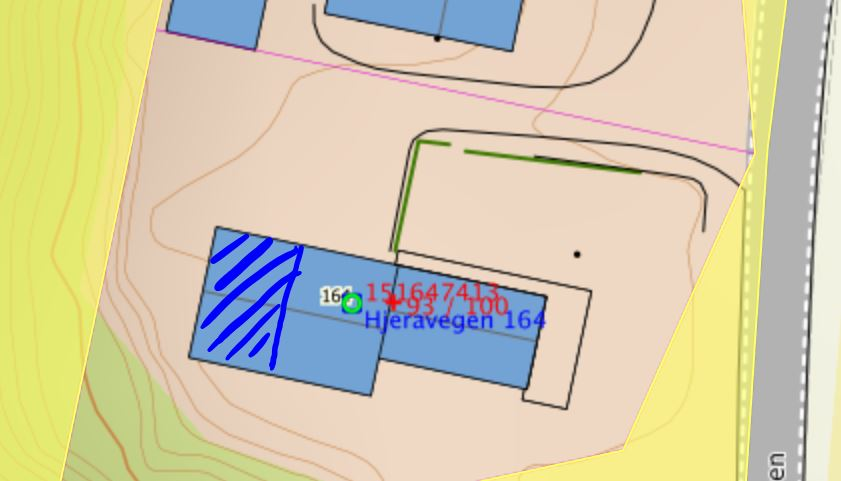
\includegraphics[width=1\textwidth]{Img/Arealskisse.JPG}
            \caption{Arealskisse over området av bygningen som leies ut. Gjelder det skraverte området}
            \label{fig:Arealskisse}
        \end{figure}


        \begin{figure}[H]
            \centering
            \includegraphics[width=1\textwidth]{Img/Utvendig.jpg}
            \caption{Lokalet utenifra}
            \label{fig:Lokalet_utenifra}
        \end{figure}


        \begin{figure}[H]
            \centering
            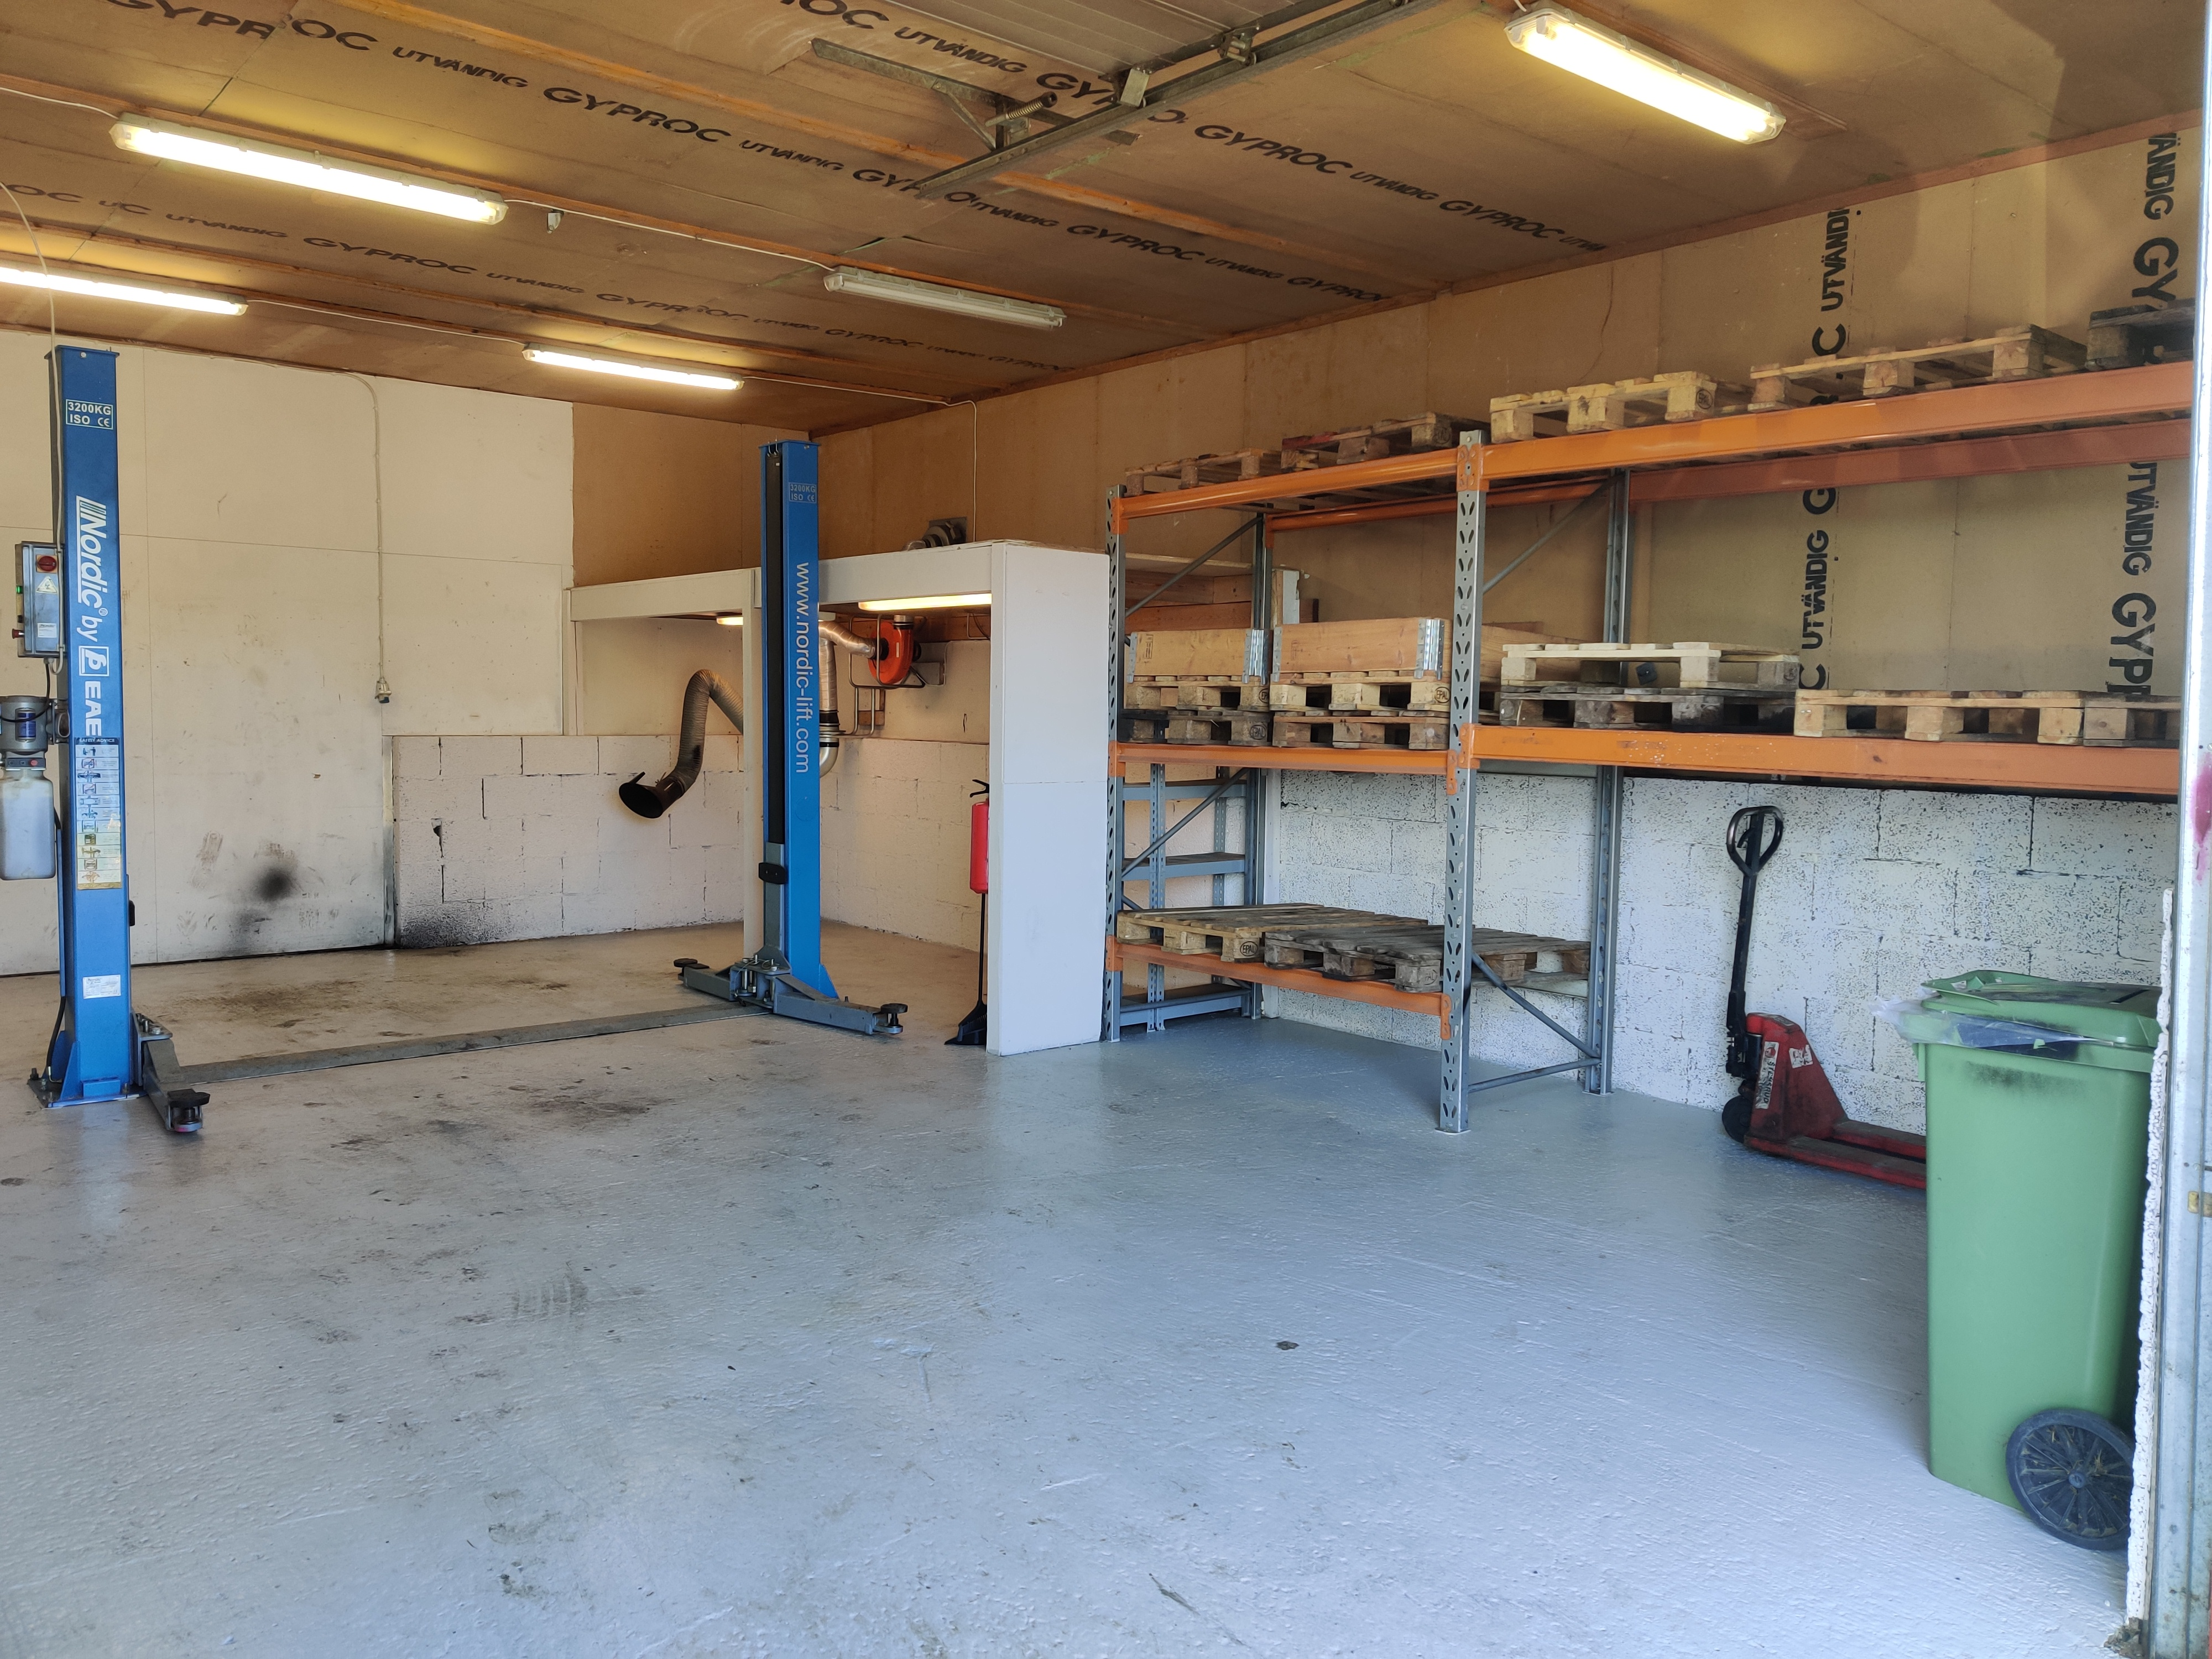
\includegraphics[width=1\textwidth]{Img/Pallereol_Og_Hems.JPG}
            \caption{Pallereol og Hems}
            \label{fig:P_og_H}
        \end{figure}


        \begin{figure}[H]
            \centering
            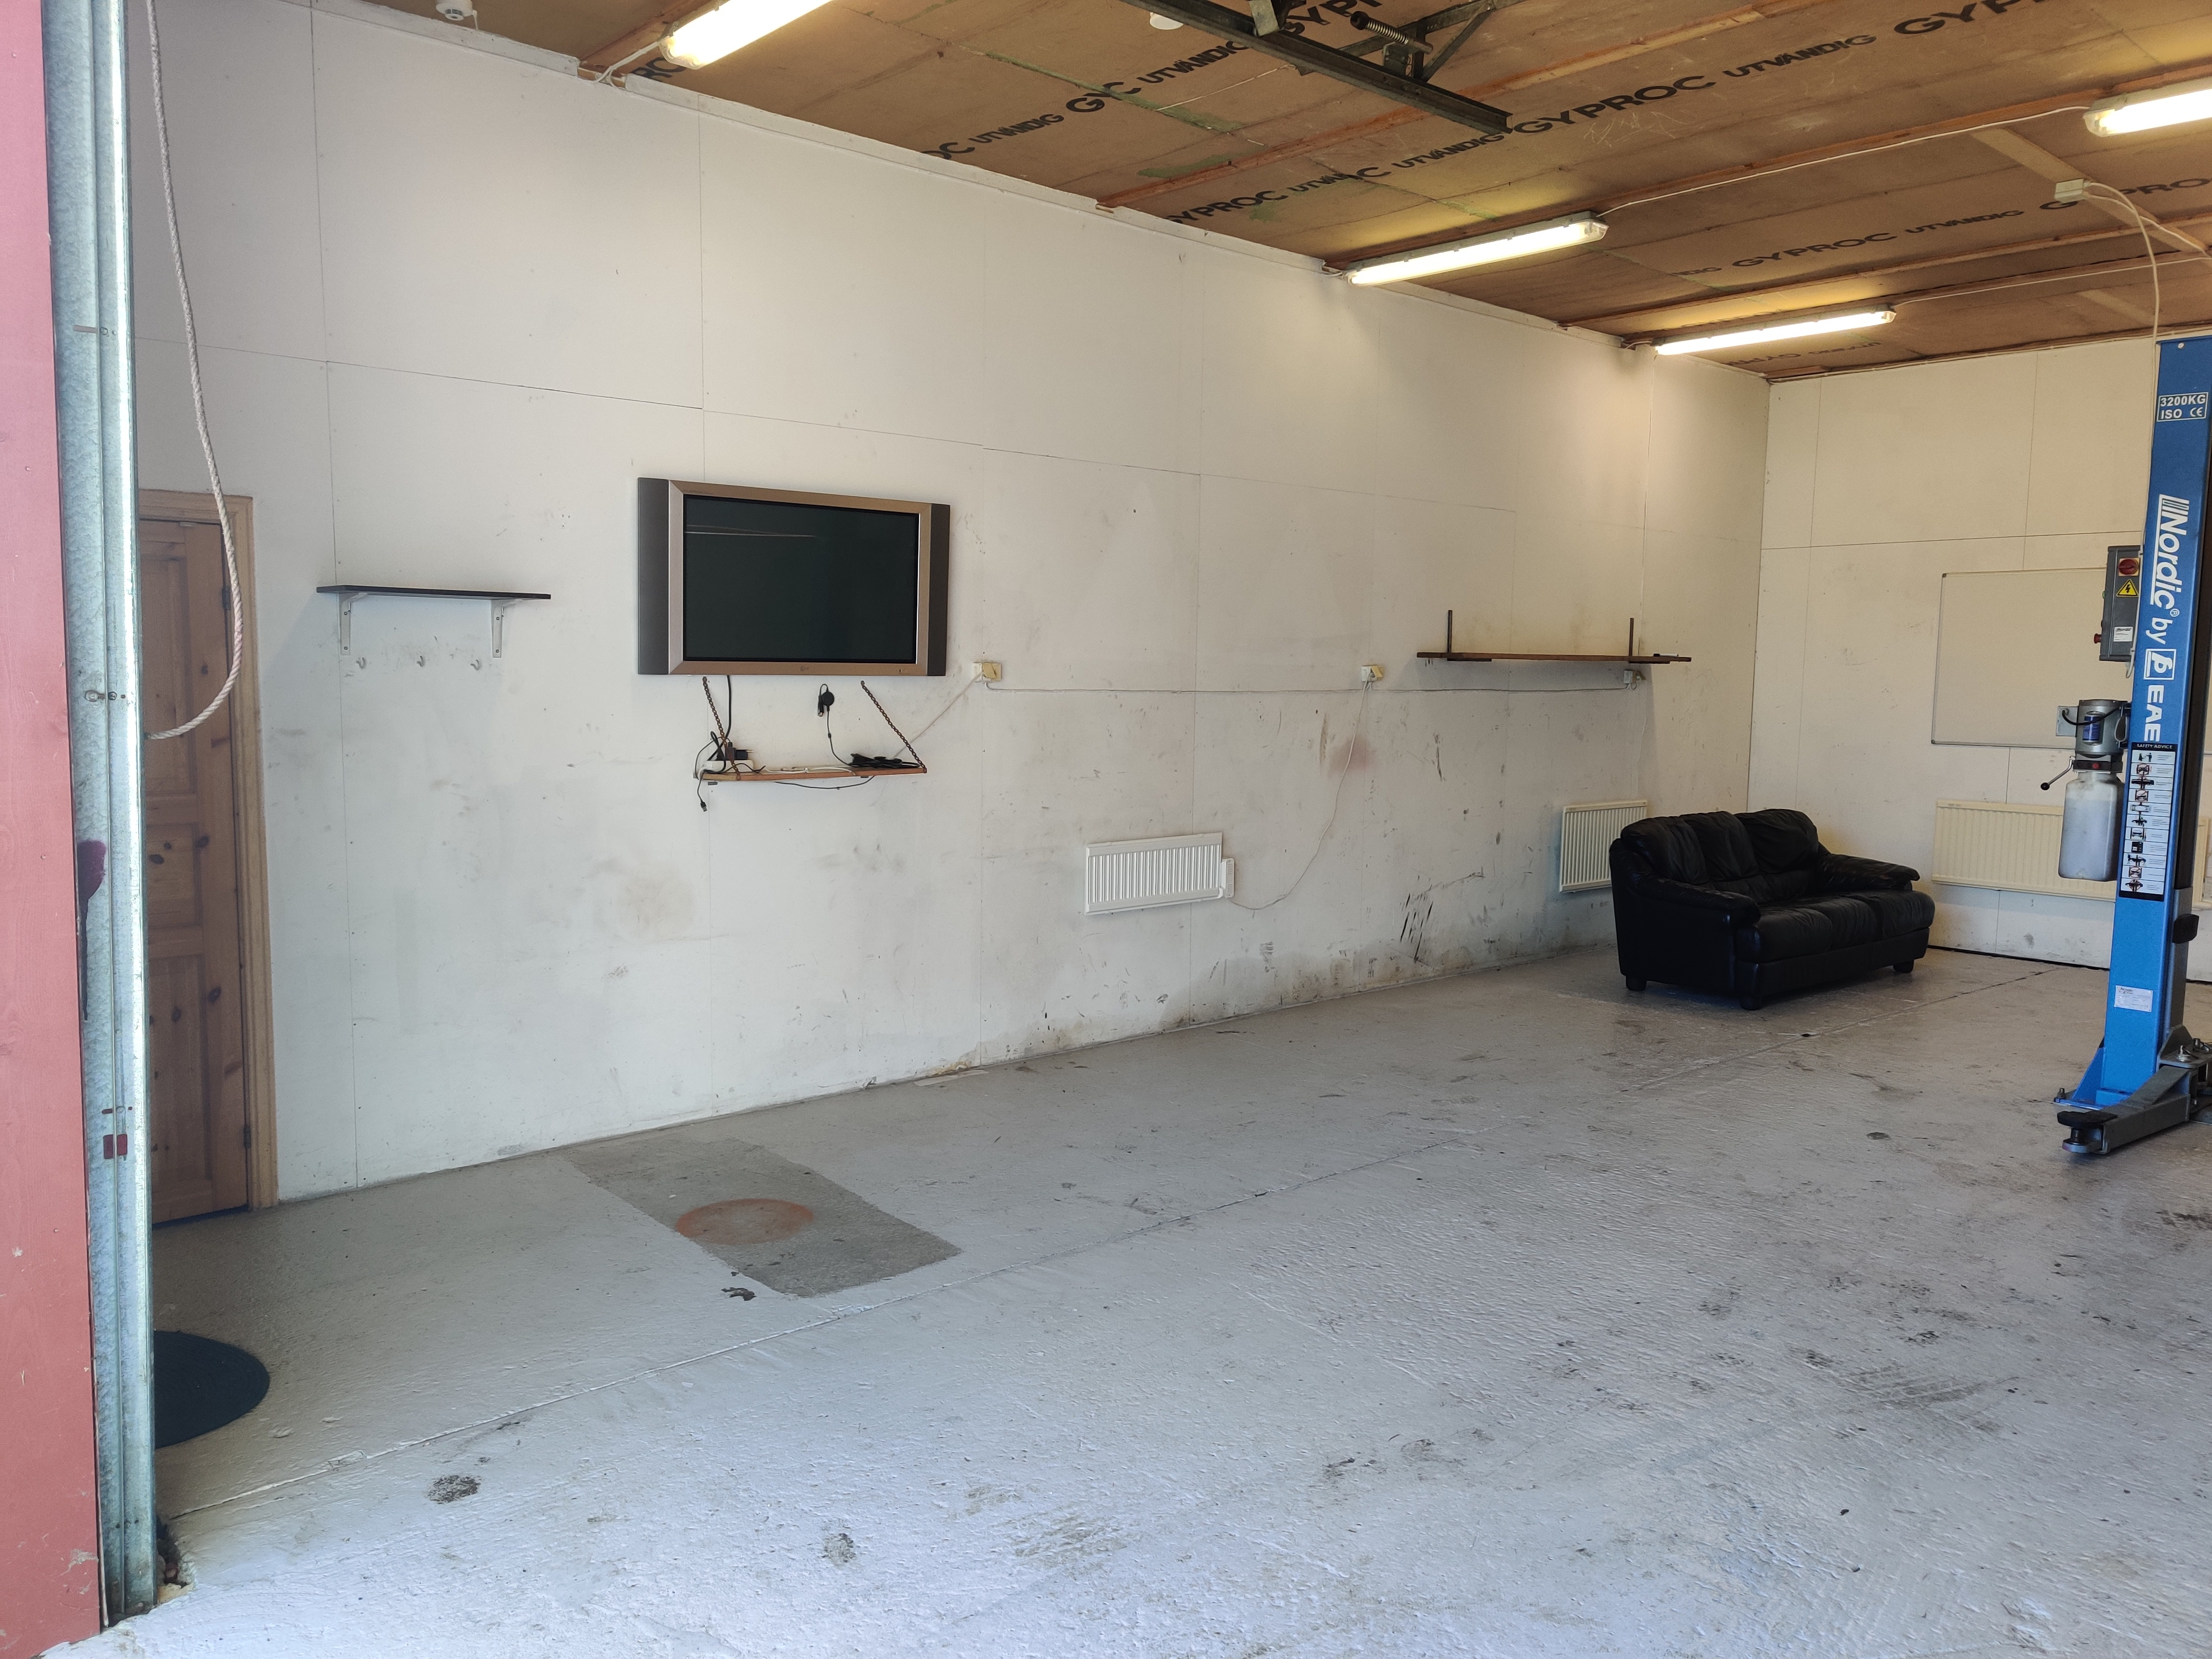
\includegraphics[width=1\textwidth]{Img/TV_Og_Sofa.JPG}
            \caption{TV og Sofa}
            \label{fig:TV_Og_Sofa}
        \end{figure}


        \begin{figure}[H]
            \centering
            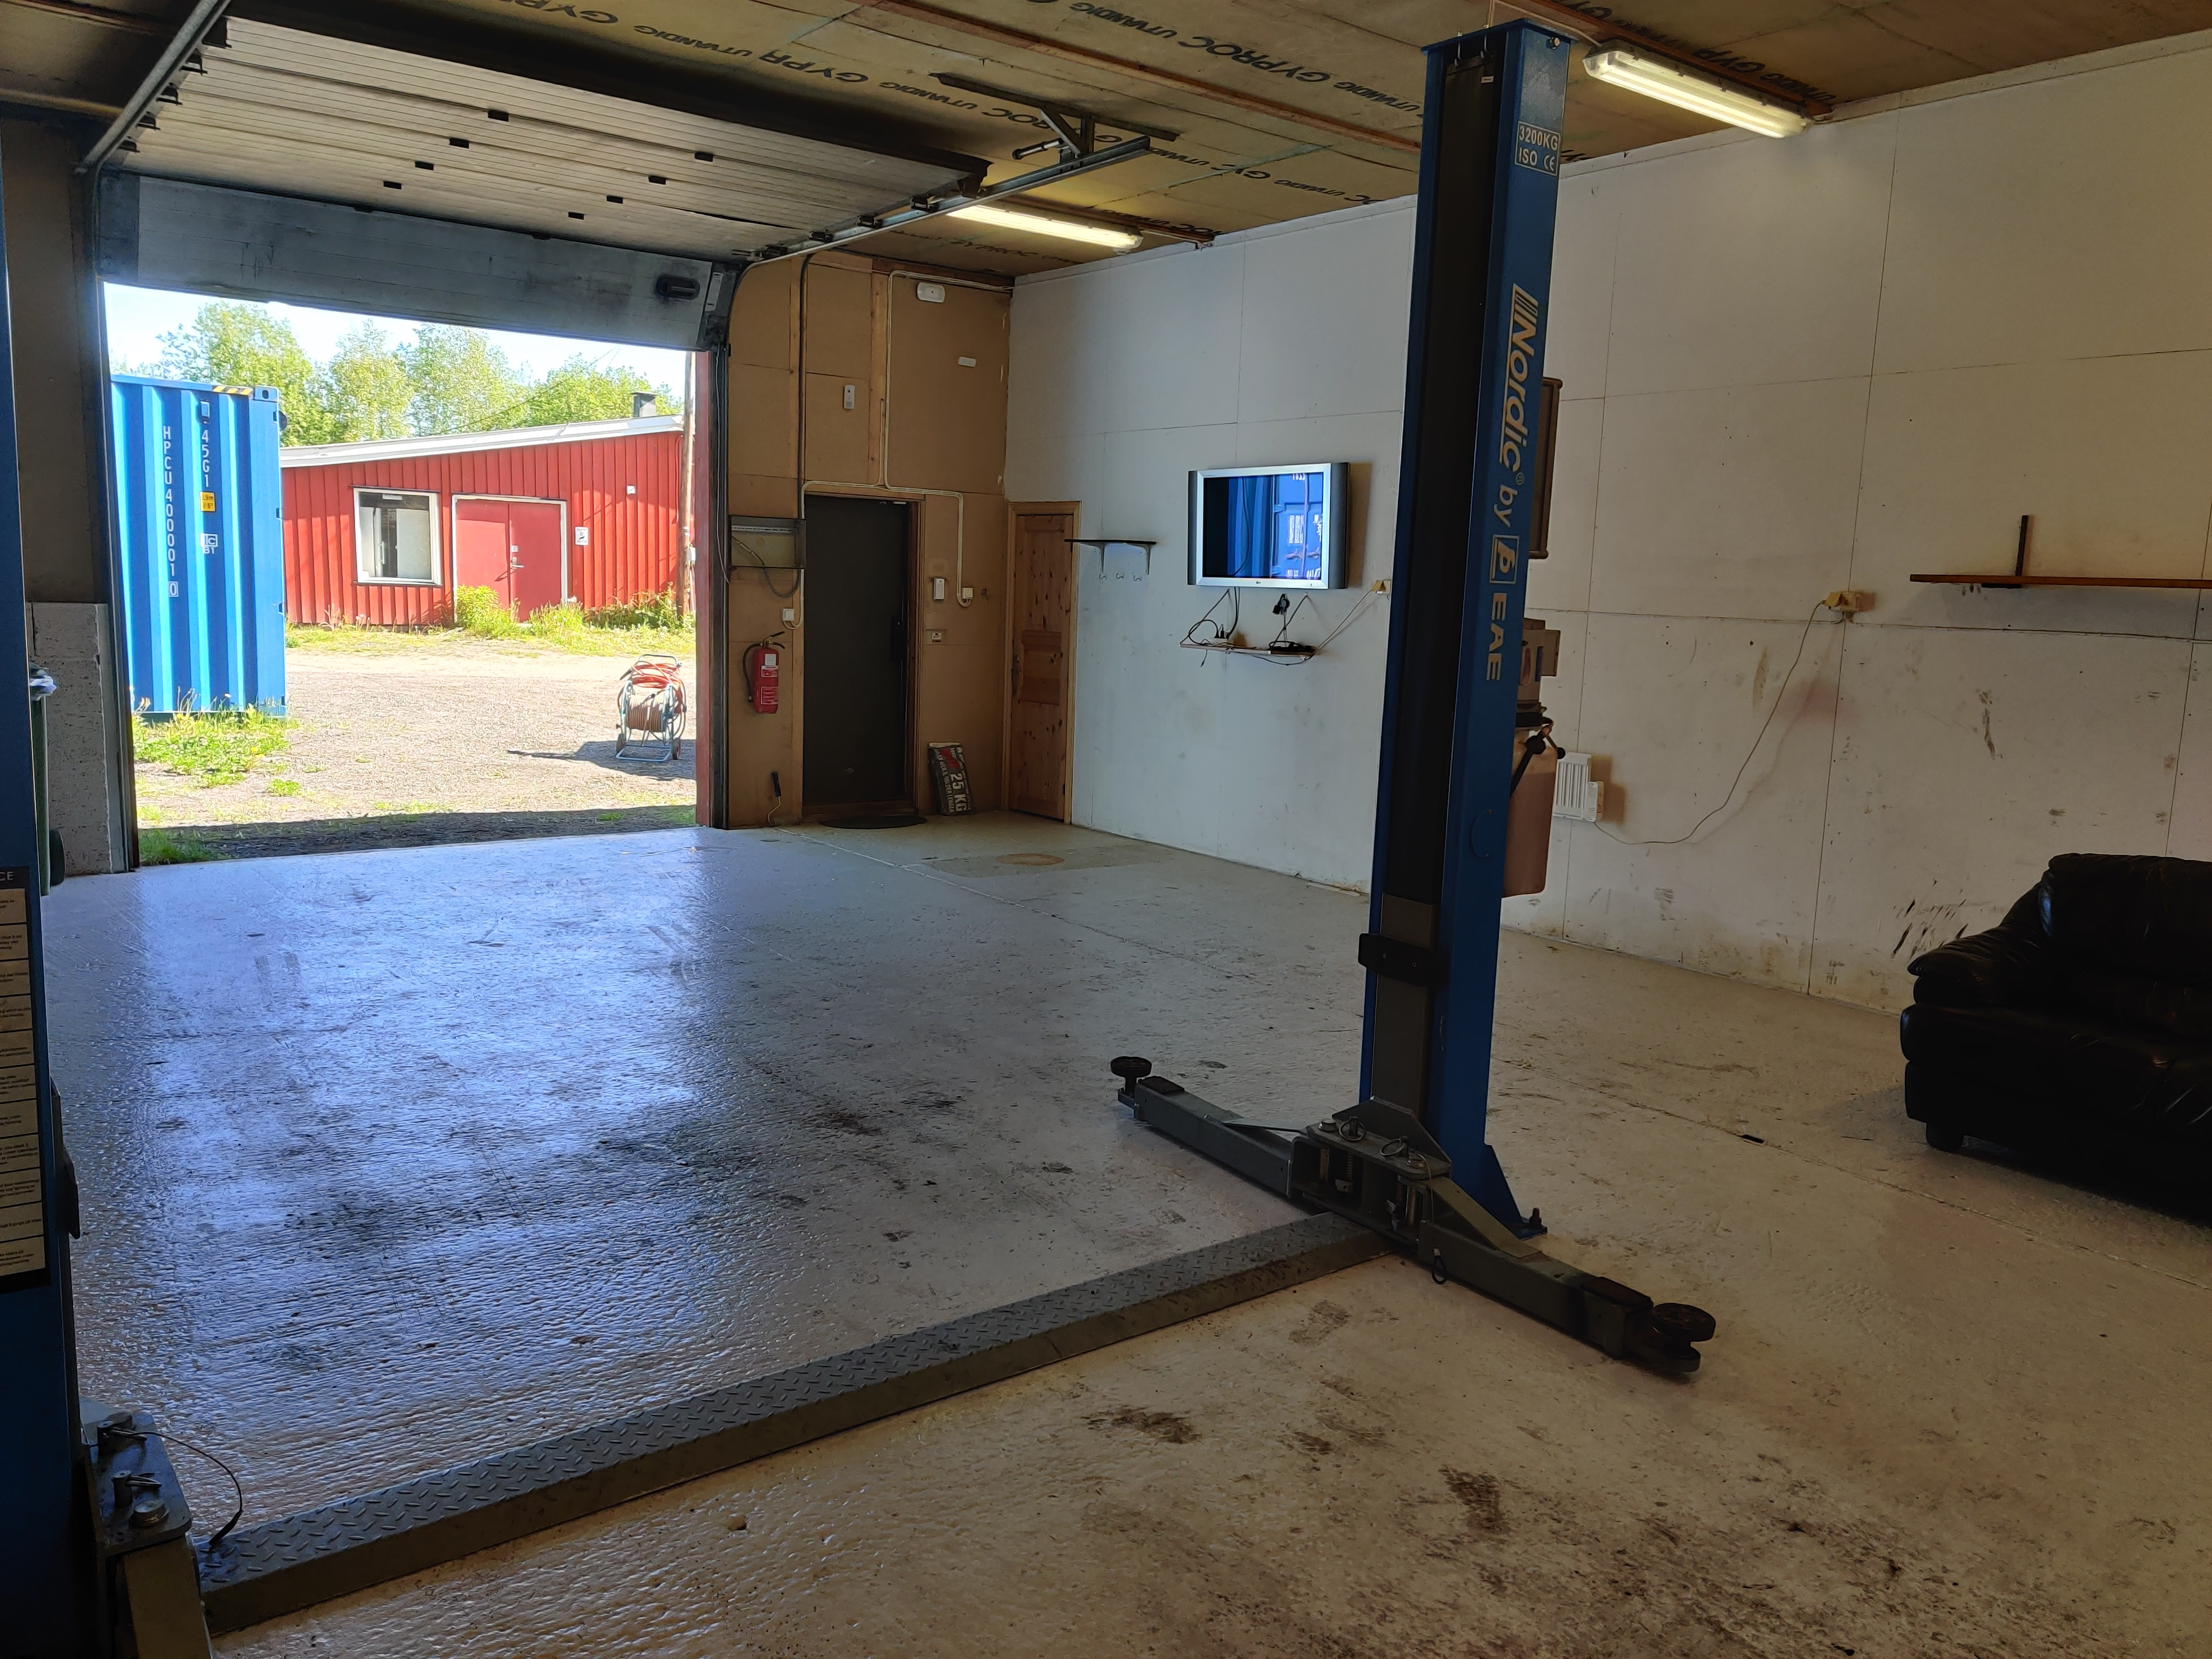
\includegraphics[width=1\textwidth]{Img/Inngang.jpg}
            \caption{Inngang og Port}
            \label{fig:Inngang}
        \end{figure}


        \begin{figure}[H]
            \centering
            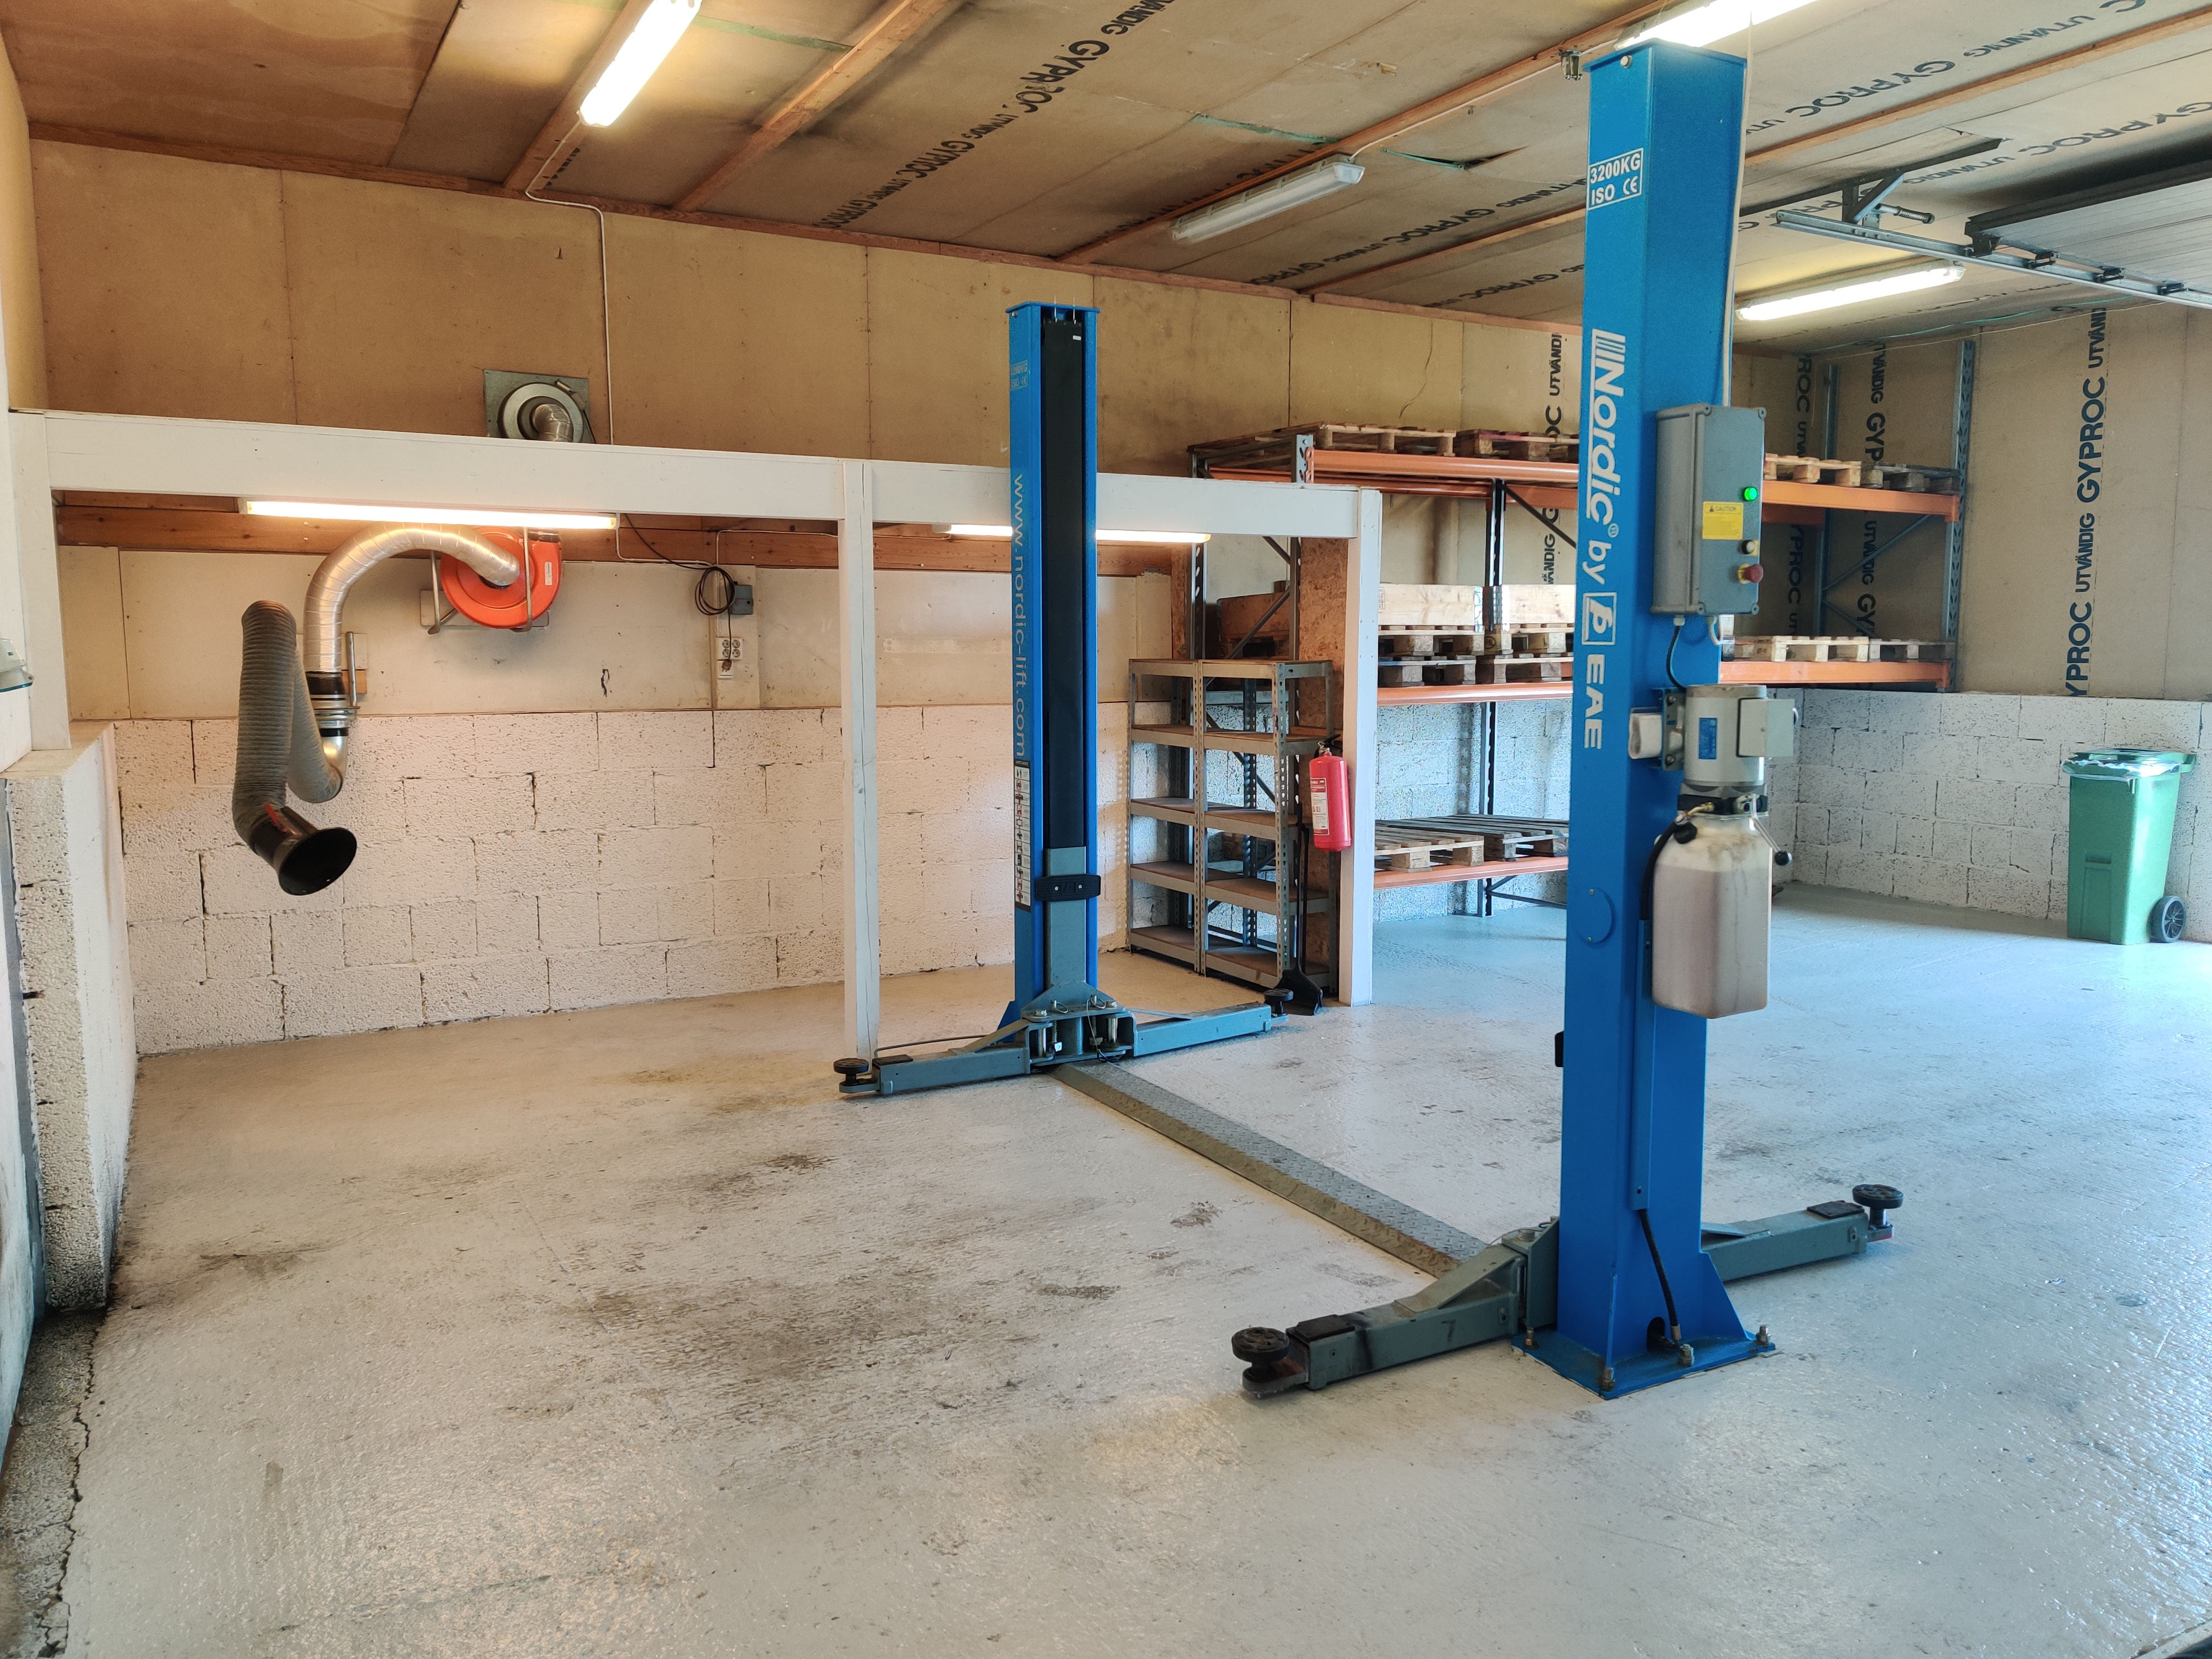
\includegraphics[width=1\textwidth]{Img/Loftebukk_Og_Punktavsug.JPG}
            \caption{Løftebukk og Punktavsug}
            \label{fig:L_og_P}
        \end{figure}



\end{document}
